\documentclass[tikz,border=1pt]{standalone}
\usepackage{newtxtext,newtxmath}
\usepackage[T1]{fontenc}
\usepackage{amsmath}
\usetikzlibrary{arrows.meta,calc}
\graphicspath{{plots/}}

% ---------------------------------------------------------------- colours
\definecolor{eorc}{HTML}{1E3A6E}   % 21-cm signal (dark blue)
\definecolor{fgc}{HTML}{A3182F}    % foregrounds (crimson red)
\definecolor{instc}{HTML}{4A5568}  % instrument / data
\definecolor{infc}{HTML}{4A5568}   % inference (same neutral grey as instrument/data)

% ------------------------------------------------------------------ styles
\tikzset{
  panel/.style={draw=#1, fill=white, line width=0.8pt,
                anchor=north west, inner sep=0pt},
  stage/.style={draw=instc, fill=white, line width=0.6pt,
                anchor=north west, inner sep=0pt,
                minimum width=2.91cm, minimum height=2.45cm},
  ttl/.style={font=\footnotesize\bfseries, align=center},
  lbl/.style={font=\footnotesize, align=center},
  small/.style={font=\scriptsize, text=black!70, align=center},
  flow/.style={-{Stealth[length=2.4mm,width=2mm]}, line width=1.1pt, draw=#1},
  flow/.default=instc,
  op/.style={font=\small, text=#1},
  op/.default=black,
  thumb/.style={inner sep=0pt},
}
\newcommand{\bm}[1]{\boldsymbol{#1}}
% \eorcube{x}{y}{size}{file prefix}: cube with front/top/side face images,
% lower-left corner of the front face at (x,y)
\newcommand{\eorcube}[4]{%
  \pgfmathsetmacro{\a}{#3}\pgfmathsetmacro{\dx}{0.38*#3}\pgfmathsetmacro{\dy}{0.265*#3}%
  \begin{scope}[shift={(#1,#2)}]
    \node[thumb, anchor=south west] at (0,0)
         {\includegraphics[width=\a cm,height=\a cm]{#4_front.png}};
    \begin{scope}[cm={1,0,\dx/\a,\dy/\a,(0,\a)}]
      \node[thumb, anchor=south west, transform shape] at (0,0)
           {\includegraphics[width=\a cm,height=\a cm]{#4_top.png}};
    \end{scope}
    \begin{scope}[cm={\dx/\a,\dy/\a,0,1,(\a,0)}]
      \node[thumb, anchor=south west, transform shape] at (0,0)
           {\includegraphics[width=\a cm,height=\a cm]{#4_side.png}};
    \end{scope}
    \draw[white, line width=0.4pt, line join=round]
         (0,0) -- (\a,0) -- (\a,\a) -- (0,\a) -- cycle
         (0,\a) -- (\dx,\a+\dy) -- (\a+\dx,\a+\dy) -- (\a,\a)
         (\a+\dx,\a+\dy) -- (\a+\dx,\dy) -- (\a,0);
  \end{scope}}

\begin{document}
\begin{tikzpicture}[x=1cm,y=1cm]

% Top row: compare model and observation, then introduce the coefficient prior.
\node[panel=infc,minimum width=6.42cm,minimum height=2.45cm] (data) at (0.45,0) {};
\draw[infc!45!panelbg,dashed,line width=0.5pt] (3.66,-0.20)--(3.66,-2.25);
\node[ttl] at (2.055,-0.25) {Modelled Data};
\node[lbl] at (2.055,-0.60) {$\bm m_{21}+\bm m_{\rm FG}$};
\node[ttl] at (5.265,-0.25) {Observed Data};
\node[lbl] at (5.265,-0.60) {$\bm d(\bm b_{ij},\nu,t)$};
% Match the model-only waterfall and observed-array panels in the other workflows.
\node[thumb] at (2.055,-1.58) {
\includegraphics[trim=1.219cm 0 0 0,clip,width=1.65cm]{icon_likelihood.pdf}};
\node[thumb] at (5.265,-1.56) {
\includegraphics{icon_array.pdf}};

\node[stage] (like) at (7.47,0) {};
\node[ttl] at (8.925,-0.25) {Full Likelihood};
\node[lbl] at (8.925,-0.59) {$\mathcal L(\bm d\mid\textcolor{eorc}{\bm a},\textcolor{fgc}{\bm q})$};
\node[thumb] at (8.925,-1.53) {
\includegraphics{icon_likelihood.pdf}};
\node[font=\scriptsize,text=instc] at (8.315,-2.17) {$\bm d$};
\node[font=\scriptsize] at (9.535,-2.17) {$\bm m$};

\node[stage] (prior) at (10.98,0) {};
\node[ttl,anchor=north] at (12.435,-0.12) {Prior\\Covariance\ \mdseries\,$\mathbf\Psi(\bm\varphi)$};
\node[thumb] at (12.485,-1.70) {
\includegraphics{icon_prior.pdf}};
\node[small,text=eorc,anchor=east] at (11.74,-1.50) {$\mathbf\Phi_{21}$};
\node[small,text=fgc,anchor=west] at (13.24,-2.12) {$\mathbf\Sigma'_{\rm FG}$};
\draw[flow] (data.east)--(like.west);
\draw[flow] (like.east)--(prior.west);

% Bottom row runs right to left, completing the inference workflow.
\node[stage] (marg) at (10.98,-3.25) {};
\node[ttl,anchor=north] at (12.435,-3.37) {Marginalised\\Likelihood\ \mdseries\,$\mathcal L(\bm d\mid\bm\varphi)$};
\node[thumb] at (12.435,-4.90) {
\includegraphics{icon_marginal.pdf}};
\draw[flow] (prior.south)--(marg.north);

\node[stage] (ns) at (7.47,-3.25) {};
\node[ttl,anchor=north] at (8.925,-3.37) {Nested\\Sampling\ \mdseries\,$\bm\rho$};
\node[thumb] at (8.925,-4.90) {
\includegraphics{icon_nested.pdf}};
\draw[flow] (marg.west)--(ns.east);

\node[panel=infc,minimum width=6.42cm,minimum height=2.45cm] (out) at (0.45,-3.25) {};
\draw[infc!45!panelbg,dashed,line width=0.5pt] (3.66,-3.45)--(3.66,-5.50);
\node[ttl,anchor=north] at (2.055,-3.37) {Power Spectrum\ \mdseries\,$\Delta^2_{21}(k)$};
\node[thumb] at (2.055,-4.72) {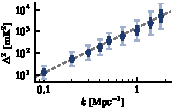
\includegraphics{icon_powerspec.pdf}};
\node[ttl,anchor=north] at (5.265,-3.37) {Bayesian Evidence\ \mdseries\,$\mathcal Z$};
\node[thumb,anchor=south] at (5.265,-5.3285) {
\includegraphics{icon_evidence.pdf}};
\node[font=\scriptsize,text=eorc,anchor=north] at (4.695,-5.33) {$\mathcal Z_{\rm21+FGs}$};
\node[font=\scriptsize,text=fgc,anchor=north] at (5.835,-5.33) {$\mathcal Z_{\rm FG}$};
\draw[flow] (ns.west)--(out.east);

\end{tikzpicture}
\end{document}
